% SPDX-License-Identifier: Apache-2.0
% yubikey-forward.tex: IEEE two-column design study (ai-coding-sop house style).
\documentclass[journal,9pt]{IEEEtran}
\usepackage{cite}
\usepackage{ifthen}
\usepackage{graphicx}
\usepackage{lmodern}
\usepackage[T1]{fontenc}
\usepackage[utf8]{inputenc}
\usepackage{microtype}
\setlength{\emergencystretch}{3em}
\usepackage{amsmath}
\usepackage{amssymb}
\usepackage{amsthm}
\usepackage{tikz}
\usetikzlibrary{arrows.meta,shapes.geometric,positioning,fit,backgrounds,calc,
                decorations.pathreplacing,matrix}
\usepackage{booktabs}
\usepackage{array}
\usepackage{multirow}
\usepackage{enumitem}
\setlist{nosep,leftmargin=*,topsep=2pt,itemsep=1pt}
\usepackage{float}
\usepackage{xcolor}
\usepackage{listings}
\usepackage[hidelinks,bookmarks=true,pdfauthor={Filip Filmar},
            pdftitle={Forwarding a YubiKey from a Chromebook to a Remote Linux Host}]{hyperref}

\theoremstyle{definition}
\newtheorem{finding}{Finding}
\newtheorem{example}{Example}[section]
\theoremstyle{remark}
\newtheorem*{tip}{Tip}
\newtheorem*{pitfall}{Pitfall}

\newcommand{\code}[1]{\texttt{#1}}
\newcommand{\term}[1]{\emph{#1}}

% Code listings: framed and highlighted; keywords bold, comments italic.
\definecolor{kwblue}{RGB}{20,60,150}
\definecolor{cmtgreen}{RGB}{90,120,90}
\definecolor{strred}{RGB}{150,50,40}
\definecolor{framegray}{gray}{0.70}
\definecolor{bgshade}{gray}{0.97}
\lstdefinestyle{go}{
  language={},
  basicstyle=\ttfamily\scriptsize,
  keywordstyle=\bfseries\color{kwblue},
  commentstyle=\itshape\color{cmtgreen},
  stringstyle=\color{strred},
  morekeywords={package,import,func,type,struct,return,if,switch,case,default,
                for,range,var,const,bool,byte,uint32,error,nil,true,false},
  morecomment=[l]{//},
  morestring=[b]",
  frame=single,
  rulecolor=\color{framegray},
  framesep=3pt,
  % Caption below, as IEEE sets figure captions. IEEEtran's \@makecaption
  % adds space only above a caption and ignores belowcaptionskip, so a
  % caption on top sits flush on the listing, and the frame (drawn
  % framesep outside the code) covers the caption's descenders.
  captionpos=b,
  % The frame reaches framesep plus the rule (about 3.4pt) outside the
  % code; pull the code in by that much, or the frame runs past the column.
  xleftmargin=3.4pt,
  xrightmargin=3.4pt,
  backgroundcolor=\color{bgshade},
  columns=fullflexible,
  keepspaces=true,
  breaklines=true,
  breakatwhitespace=true,
}
\lstdefinestyle{shell}{
  basicstyle=\ttfamily\scriptsize,
  keywordstyle=\ttfamily,
  commentstyle=\itshape\color{cmtgreen},
  stringstyle=\ttfamily,
  morecomment=[l]{\#},
  frame=single,
  rulecolor=\color{framegray},
  framesep=3pt,
  % Caption below, as IEEE sets figure captions. IEEEtran's \@makecaption
  % adds space only above a caption and ignores belowcaptionskip, so a
  % caption on top sits flush on the listing, and the frame (drawn
  % framesep outside the code) covers the caption's descenders.
  captionpos=b,
  % The frame reaches framesep plus the rule (about 3.4pt) outside the
  % code; pull the code in by that much, or the frame runs past the column.
  xleftmargin=3.4pt,
  xrightmargin=3.4pt,
  backgroundcolor=\color{bgshade},
  columns=fullflexible,
  keepspaces=true,
  breaklines=true,
}

\tikzset{
  box/.style={draw,rounded corners=1pt,align=center,inner sep=3pt,
              minimum height=6.5mm,font=\footnotesize},
  sbox/.style={box,fill=blue!7},
  act/.style={box,fill=green!12},
  mem/.style={box,fill=orange!12},
  warnb/.style={box,fill=red!8},
  ghost/.style={box,fill=black!5},
  fl/.style={-{Stealth[length=4pt]},shorten >=2.5pt,shorten <=2.5pt},
  fld/.style={-{Stealth[length=4pt]},dashed,shorten >=2.5pt,shorten <=2.5pt},
  bidi/.style={{Stealth[length=4pt]}-{Stealth[length=4pt]},shorten >=2.5pt,shorten <=2.5pt},
}

% ---------------------------------------------------------------------------
\title{Forwarding a YubiKey from a Chromebook\\to a Remote Linux Host\\{\large A Design Study}}

\author{Filip Filmar%
\thanks{This paper is a design study, not a product description.
It compares the ways to use a YubiKey that is plugged into a Chromebook
from a remote Linux host, and recommends one.
The running example is one WebAuthn login in Chrome on the remote host,
which the user reaches through Chrome Remote Desktop.
Every claim about software is marked as verified, with its source, or as an
assumption. The decisive claim was tested on one Chromebook with a U2F
security key; the test plan and its results are in
Section~\ref{sec:testplan}.}}

\markboth{Design study~~$\cdot$~~November 2026}{YubiKey forwarding from a Chromebook}

\begin{document}
\maketitle

\begin{abstract}
A user works on a remote Linux desktop through Chrome Remote Desktop, from a
Chromebook. The user's YubiKey is plugged into the Chromebook. Chrome Remote
Desktop does not forward security keys, so web logins that need the key fail
on the remote desktop. This study compares eleven ways to make the key usable
on the remote host. They include a userspace USB/IP server, a relay of FIDO
HID reports over SSH, virtual FIDO devices, agent forwarding, a WebAuthn
proxy extension, and smart card relays. The study finds one fact that decides
the design: the ChromeOS Linux container receives a shared USB device only as
a raw usbfs node, never as a \code{hidraw} node. Existing relays need
\code{hidraw}. We recommend a relay of FIDO HID reports over SSH, with a new
key-side component that reads the key through usbfs and refuses commands that
can erase the key. We recommend agent forwarding for OpenPGP and PIV. A probe on a real
Chromebook confirmed that the container can claim a security key's FIDO
interface and talk to it in 3\,ms.
\end{abstract}

\begin{IEEEkeywords}
FIDO2, WebAuthn, CTAPHID, YubiKey, ChromeOS, Crostini, usbfs, uhid, USB/IP,
SSH, remote desktop, security keys
\end{IEEEkeywords}

{\footnotesize\tableofcontents}

% SPDX-License-Identifier: Apache-2.0
\section{Introduction}
\label{sec:intro}

\IEEEPARstart{M}{any} engineers work on a remote Linux desktop from a
Chromebook. Chrome Remote Desktop (CRD) shows the remote screen and sends the
keyboard and the mouse. It does not send USB devices, and it does not send
security keys. A web login that asks for a security key therefore fails on
the remote desktop, even when the key is plugged into the Chromebook in front
of the user.

This study looks for a way to use that key on the remote host. It does not
change CRD. Google's internal CRD client can proxy WebAuthn, but that path is
closed to everyone else (Section~\ref{sec:approaches}).

\subsection{The setting}

The local machine is a Chromebook in normal mode. The user cannot load kernel
modules and does not use developer mode. The user runs the Linux development
environment, which ChromeOS calls Crostini. ChromeOS can share a USB device
with that environment through \term{Manage USB devices}.

The remote machine runs Linux. The user has root there, and reaches it by CRD
and by SSH.

The goals, in priority order:
\begin{enumerate}
\item WebAuthn and FIDO2 in Chrome on the remote host.
\item SSH with FIDO keys (\code{ed25519-sk}), OpenPGP, and PIV on the remote
      host. These are nice to have.
\end{enumerate}

\subsection{The running example}

One login runs through the whole paper. The user opens a web site in Chrome
inside the CRD session on the remote host. The site asks for a passkey. Chrome
on the remote host must find a FIDO authenticator, send it a
\code{getAssertion} request, and get back a signature that the real YubiKey
made after a touch on the Chromebook.

\subsection{Contributions}

\begin{itemize}
\item A comparison of eleven approaches (Section~\ref{sec:comparison}).
\item One decisive fact from the ChromeOS source: the Linux container gets a
      shared USB device only as a usbfs node, with no \code{hidraw} node
      (Section~\ref{sec:crostini}).
\item A recommended design that reuses an existing relay and adds one small
      component (Sections~\ref{sec:recommendation} and~\ref{sec:component}).
\item A probe and a test plan for the real Chromebook
      (Section~\ref{sec:testplan}).
\end{itemize}

\subsection{How to read this paper}

Section~\ref{sec:background} explains the YubiKey's USB interfaces and the
CTAPHID protocol. Section~\ref{sec:crostini} explains how ChromeOS shares a
USB device with Linux. If you know both, start at
Section~\ref{sec:approaches}. Each claim about other software is marked
\term{verified}, with a source, or \term{assumption}.

% SPDX-License-Identifier: Apache-2.0
\section{Background}
\label{sec:background}

\subsection{The YubiKey's USB interfaces}

A YubiKey 5 shows three USB interfaces to the host~\cite{yk-usb}
(verified). Table~\ref{tab:interfaces} lists them. Each interface is a
separate unit for the host's drivers. A process can claim one interface and
leave the others to other drivers.

\begin{table}[t]
\centering
\caption{YubiKey 5 USB interfaces}
\label{tab:interfaces}
\scriptsize
\begin{tabular}{@{}l>{\raggedright\arraybackslash}p{17mm}>{\raggedright\arraybackslash}p{15mm}>{\raggedright\arraybackslash}p{23mm}@{}}
\toprule
Interface & Class & Endpoints & Functions \\
\midrule
OTP & HID keyboard & interrupt IN & Yubico OTP, static password \\
FIDO & HID, usage page 0xF1D0 & interrupt IN and OUT & U2F, FIDO2 \\
CCID & smart card & bulk IN and OUT & PIV, OpenPGP, OATH \\
\bottomrule
\end{tabular}
\end{table}

The goals of Section~\ref{sec:intro} map onto the interfaces. WebAuthn needs
only the FIDO interface. OpenPGP and PIV need the CCID interface. The OTP
interface is not a goal.

\subsection{CTAPHID}

A FIDO key on USB talks CTAPHID~\cite{ctap21}. CTAPHID cuts each message into
64-byte HID reports. Figure~\ref{fig:packets} shows the two packet kinds. The
first packet holds the channel ID (CID), the command, and the payload length.
Each continuation packet holds the CID and a sequence number. One message can
hold up to 7609 bytes: 57 bytes in the first packet and 59 bytes in each of
128 continuation packets.

\begin{figure}[t]
\centering
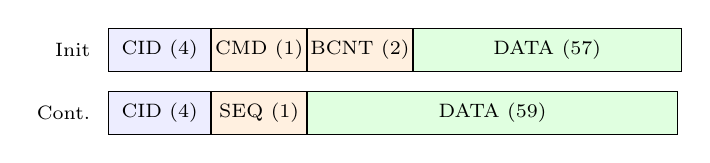
\begin{tikzpicture}[font=\scriptsize]
  \tikzset{fld/.style={draw,minimum height=5.5mm,inner sep=1pt,anchor=west}}
  \node[anchor=east] at (-1mm,0) {Init};
  \node[fld,fill=blue!7,minimum width=13mm] (a) at (0,0) {CID (4)};
  \node[fld,fill=orange!12,minimum width=12mm] (b) at (a.east) {CMD (1)};
  \node[fld,fill=orange!12,minimum width=13mm] (c) at (b.east) {BCNT (2)};
  \node[fld,fill=green!12,minimum width=34mm] at (c.east) {DATA (57)};
  \node[anchor=east] at (-1mm,-8mm) {Cont.};
  \node[fld,fill=blue!7,minimum width=13mm] (d) at (0,-8mm) {CID (4)};
  \node[fld,fill=orange!12,minimum width=12mm] (e) at (d.east) {SEQ (1)};
  \node[fld,fill=green!12,minimum width=47mm] at (e.east) {DATA (59)};
\end{tikzpicture}
\caption{The two CTAPHID packet kinds. Each is one 64-byte HID report. Field
sizes are in bytes; the boxes are not to scale. In an init packet, bit 7 of
CMD is set.}
\label{fig:packets}
\end{figure}

A client first sends \code{CTAPHID\_INIT} on the broadcast channel
\code{0xFFFFFFFF} with an 8-byte nonce. The key replies with a new channel
ID. All later messages use that channel. FIDO2 requests travel as
\code{CTAPHID\_CBOR} messages. The first payload byte names the CTAP2
command. For example, \code{0x02} is \code{getAssertion} and \code{0x07} is
\code{reset}.

While the key waits for a touch, it sends \code{CTAPHID\_KEEPALIVE} at least
every 100\,ms~\cite{ctap21} (verified). Chrome on Linux waits 20\,s for a
FIDO device, and each keepalive starts that wait again~\cite{chromefido}
(verified). A relay that passes keepalives through therefore has no hard
time limit for the touch.

\subsection{Linux devices for HID}

On a normal Linux host the kernel driver \code{usbhid} binds to each HID
interface. It creates one \code{/dev/hidrawN} node per interface. Chrome,
libfido2, and OpenSSH all find FIDO keys through these nodes. Chrome uses any
HID device that declares usage page \code{0xF1D0}, on any bus~\cite{chromefido}
(verified).

The kernel module \code{uhid} lets a userspace process create a HID device.
The process writes a report descriptor to \code{/dev/uhid}. The kernel then
creates a new \code{hidraw} node for it. A relay can use this to make a
\term{virtual} FIDO key on the remote host.

Below \code{hidraw} is \term{usbfs}: one node per USB device under
\code{/dev/bus/usb}. A process that opens it can read the descriptors, detach
the kernel driver from an interface, claim the interface, and run transfers
with \code{ioctl} calls. libusb uses usbfs on Linux.

% SPDX-License-Identifier: Apache-2.0
\section{How ChromeOS shares a USB device with Linux}
\label{sec:crostini}

Crostini is a stack of three layers. ChromeOS runs a virtual machine,
\code{termina}, with crosvm. Inside \code{termina}, an LXD container named
\code{penguin} holds the user's Debian system. Figure~\ref{fig:crostini}
shows the path that a shared USB device takes.

\begin{figure}[t]
\centering
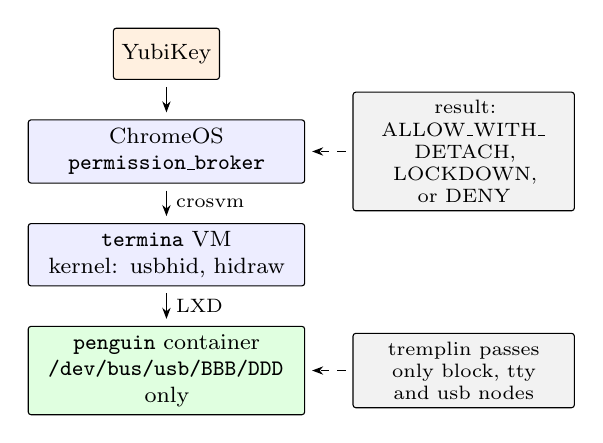
\begin{tikzpicture}[node distance=5mm and 4mm]
  \node[mem] (yk) {YubiKey};
  \node[sbox,below=of yk,text width=33mm] (pb) {ChromeOS\\\code{permission\_broker}};
  \node[sbox,below=of pb,text width=33mm] (vm) {\code{termina} VM\\kernel: usbhid, hidraw};
  \node[act,below=of vm,text width=33mm] (ct) {\code{penguin} container\\\code{/dev/bus/usb/BBB/DDD} only};
  \node[ghost,right=6mm of pb,text width=26mm,font=\scriptsize] (dec)
       {result:\\ALLOW\_WITH\_\\DETACH, LOCKDOWN,\\or DENY};
  \node[ghost,right=6mm of ct,text width=26mm,font=\scriptsize] (tr)
       {tremplin passes only block, tty and usb nodes};
  \draw[fl] (yk) -- (pb);
  \draw[fl] (pb) -- node[right,font=\scriptsize]{crosvm} (vm);
  \draw[fl] (vm) -- node[right,font=\scriptsize]{LXD} (ct);
  \draw[fld] (dec) -- (pb);
  \draw[fld] (tr) -- (ct);
\end{tikzpicture}
\caption{The path of a shared USB device. The container receives only the
usbfs node. The \code{hidraw} nodes stay in the VM.}
\label{fig:crostini}
\end{figure}

\subsection{ChromeOS can refuse the key}

When the user turns on sharing, Chrome asks \code{permission\_broker} for all
interfaces of the device~\cite{crosusb} (verified). The broker's rule for
conforming devices returns one of three results~\cite{pb} (verified). A
device that ChromeOS tags as external gets \code{ALLOW\_WITH\_DETACH}. A
device in the older flow, with \code{usbhid} bound, gets
\code{ALLOW\_WITH\_LOCKDOWN} or \code{DENY}. A 2025 report shows a YubiKey
that got \code{DENY} on a new Chromebook and \code{ALLOW\_WITH\_DETACH} on an
older one. Turning off the Smart Card Connector app fixed the new
one~\cite{cros-scc} (verified).

\begin{pitfall}
The result depends on the Chromebook model and on the apps that are
installed. Test T1 (Section~\ref{sec:testplan}) checks it first, because a
refusal ends approaches A and B on that Chromebook.
\end{pitfall}

\subsection{The container gets no \code{hidraw} node}

\begin{finding}
\label{find:nohidraw}
The \code{penguin} container receives a shared USB device only as its usbfs
node, \code{/dev/bus/usb/BBB/DDD}, with mode \code{0666}. It receives no
\code{hidraw} node. The container manager, tremplin, passes only the uevents
of the subsystems block, tty and usb into the container~\cite{tremplin}
(verified, two independent reads of the source).
\end{finding}

This finding decides the design. Every existing FIDO relay that we found
reads the key through \code{hidraw}: fido-forward, qubes-app-u2f through
python-fido2, and auth-relay through python-fido2. libfido2, and so OpenSSH's
FIDO support, also needs \code{hidraw}. None of them can see the key inside
\code{penguin}.

\begin{finding}
\label{find:detach}
A process that has a usbfs node open can detach the kernel driver from one
interface. The kernel performs no capability check for this
\code{ioctl}~\cite{devio} (verified).
\end{finding}

Together, Findings~\ref{find:nohidraw} and~\ref{find:detach} suggest that a
process in \code{penguin} can detach \code{usbhid} from the FIDO interface,
claim it, and talk CTAPHID through usbfs. Nobody has reported this yet
(assumption). The probe in Section~\ref{sec:testplan} tests it.

\subsection{The key cannot serve both sides}

A key that is shared with Crostini is not available to Chrome on the
Chromebook. One 2025 report says that sharing takes an exclusive lock, so
passkeys stop working in the ChromeOS browser~\cite{crosvmdev} (verified, one
report). ChromeOS has a second path, \code{vmc key-attach}, which shares the
key with both sides. It supports U2F only, and FIDO2 traffic
hangs~\cite{crosvmdev} (verified, the maintainer confirmed it).

% SPDX-License-Identifier: Apache-2.0
\section{Approaches}
\label{sec:approaches}

This section describes each approach and what we found about it.
Section~\ref{sec:comparison} compares them in one table.

\subsection{Userspace USB/IP server in Crostini (A)}

USB/IP sends USB transfers over TCP. A userspace server in \code{penguin}
opens the key with libusb and exports it. The remote host loads
\code{vhci-hcd} and runs \code{usbip attach} through an SSH tunnel. The remote
host then sees the whole key, with all three interfaces.

Two servers can export a real device. jiegec/usbip~\cite{jiegec} (Rust, MIT)
runs one blocking transfer at a time, with a fixed 1\,s timeout, and answers
a cancel request without cancelling anything (verified, source). A YubiKey
report against it, issue~51, closed with no fix (verified).
yunsmall/usbipdcpp~\cite{usbipdcpp} (C++, LGPL-3.0) submits transfers
asynchronously and cancels them correctly (verified, source). It is less than
two years old, and nobody has reported it with a YubiKey (assumption: unknown
maturity). The remote side needs \code{vhci-hcd}, which Debian and Ubuntu
ship as a module~\cite{usbip-deb} (verified).

\subsection{CTAPHID relay with uhid (B)}

A relay moves the 64-byte CTAPHID reports between the real key and a virtual
FIDO key that \code{uhid} creates on the remote host. SSH carries the
reports.

fido-forward~\cite{fidoforward} (Go, MIT) does this. Its key side opens
\code{/dev/hidrawN}. Its remote side, the \term{sink}, runs setuid to a
dedicated user, opens \code{/dev/uhid}, and drops privilege before it reads
any input (verified, source and requirements). Its wire format is a 5-byte
marker, \code{FFWD} and version \code{0x01}, in each direction, then raw
64-byte reports (verified). It filters CTAPHID channels, but not CTAP
commands. The project is one month old and has one author.

qubes-app-u2f~\cite{qubes} (Python, GPL-2.0+) relays parsed CTAP messages,
not raw reports, over Qubes qrexec. It passes only four CTAP2 commands and
sends no keepalives (verified, source). Chromium times out after a PIN
prompt with it, and libfido2 cannot detect it (verified, open issues).

\subsection{Virtual FIDO device with delegated crypto (C)}

A software authenticator on the remote host could send only its signing step
to the real key. This does not work. A real key never exports its private
key, and it signs data that it builds itself: the relying party hash, the
flags, and the counter. bulwarkid/virtual-fido~\cite{virtualfido} signs
inside the library with a Go key (verified, \code{ctap/ctap.go} lines 250 and
364). Delegating to a real key means forwarding whole CTAP commands, which
is approach~B.

\subsection{Agent forwarding (D)}

OpenSSH's agent signs locally, and a forwarded agent lets the remote host ask
for signatures~\cite{openssh} (verified). The FIDO touch happens on the local
key. Since OpenSSH 8.4, a forwarded agent refuses to sign WebAuthn challenges
with FIDO keys~\cite{openssh} (verified), so agent forwarding cannot serve
goal~1. gpg-agent has an \term{extra socket} for forwarding, which refuses
key export and most card commands~\cite{gnupgfwd} (verified). p11-kit can
forward a PKCS\#11 token, such as the YubiKey's PIV applet, over a Unix
socket and SSH~\cite{p11kit} (verified).

In Crostini, users report that \code{pcscd} and \code{gpg} work with a shared
key (verified, two reports). FIDO keys for SSH do not work there, because
libfido2 needs \code{hidraw} (Finding~\ref{find:nohidraw}).

\subsection{Other approaches (E1 to E6)}

\paragraph{E1. Hybrid transport} Chrome can use a phone as authenticator.
The hybrid transport needs a Bluetooth advertisement near the
client~\cite{ctap22} (verified). A remote host has no phone nearby.

\paragraph{E2. CRD forwarding} Chromium has code to proxy security keys and
WebAuthn through CRD. Its policies are internal to Google, or for managed
users only, and the WebAuthn channel accepts only the official CRD extension
IDs~\cite{crdpol} (verified).

\paragraph{E3. WebAuthn proxy extension} The extension API
\code{chrome.webAuthenticationProxy} lets an extension take over WebAuthn in
Chrome~\cite{wap} (verified). auth-relay~\cite{authrelay} uses it on the
remote host and sends CTAP2 requests over SSH to python-fido2 on the laptop.
The proxied request has no origin field, so auth-relay guesses the origin
from the active tab (verified, source). Its laptop side needs \code{hidraw}.

\paragraph{E4. Smart card relay} vsmartcard~\cite{vsmartcard} (GPL-3.0)
relays a local PC/SC card to a virtual reader on another host (verified). It
can carry PIV and OpenPGP (assumption: untested with a YubiKey). The remote
host can then send any APDU to the card.

\paragraph{E5. Log in on the Chromebook} The Chromebook's own Chrome can open
a web app that the remote host serves, through an SSH SOCKS proxy. The host
name stays the same, so the relying party ID matches~\cite{webauthn3}
(assumption for the proxy setup). This avoids forwarding, but it does not help
when the login must happen inside the remote desktop.

\paragraph{E6. \code{vmc key-attach}} It shares the key with ChromeOS and
Linux at once, but only for U2F~\cite{crosvmdev} (verified). Passkeys need
FIDO2.

% SPDX-License-Identifier: Apache-2.0
\section{Comparison}
\label{sec:comparison}

Table~\ref{tab:compare} compares the approaches. ``Crostini'' means that the
approach works in Crostini with no root on ChromeOS, no kernel module, and no
developer mode. ``Both'' means that the key works on the Chromebook and on the
remote host at the same time.

\begin{table*}[t]
\centering
\caption{Comparison of the approaches. Y: yes. N: no. P: partly. ``a'' marks an assumption.}
\label{tab:compare}
\scriptsize
\setlength{\tabcolsep}{3pt}
\begin{tabular}{@{}p{24mm}p{30mm}ccccccp{38mm}p{30mm}@{}}
\toprule
Approach & Existing software & FIDO2 & OTP & PIV & PGP & Crostini & Both & Main security risk & Timeout risk \\
\midrule
A. USB/IP from Crostini & jiegec/usbip (serial, bug \#51); usbipdcpp (async) & Y\,a & Y\,a & Y\,a & Y\,a & P & N & Remote root has raw USB to all applets: reset, PIN exhaustion, OTP changes. No transport authentication. & High for jiegec/usbip; low for usbipdcpp (a) \\
B. CTAPHID relay, uhid & fido-forward (remote side as is); new usbfs key side & Y & N & N & N & P & N & Remote asks for assertions for any site. Reset and credential management blocked by the new policy. & Low: keepalives pass \\
B$'$. qubes-app-u2f over SSH & qubes-app-u2f & P & N & N & N & N & N & Built-in command filter & High: no keepalives \\
C. Virtual device, delegated crypto & virtual-fido, tpm-fido & N & N & N & N & -- & -- & Not possible: a real key cannot sign for it & -- \\
D. Agent forwarding & OpenSSH, GnuPG, p11-kit & N & N & Y & Y & P & N & Remote uses the agent while the session is open & Low \\
E1. Hybrid (phone) & Chrome & phone & N & N & N & -- & Y & Low & Needs Bluetooth at the remote host \\
E2. CRD forwarding & CRD & internal & N & N & N & -- & -- & -- & Not available \\
E3. WebAuthn proxy extension & auth-relay & Y\,a & N & N & N & N & N & No origin in the proxied request; origin is guessed & Low \\
E4. Smart card relay & vsmartcard & N & N & Y\,a & Y\,a & P & N & Remote sends any APDU & Low (a) \\
E5. Chromebook Chrome via SOCKS & Chrome, OpenSSH & Y & N & N & N & Y & Y & Low: the key stays local & Low; only for web apps the remote serves \\
E6. \code{vmc key-attach} & ChromeOS & U2F & N & N & N & P & Y & As B & No FIDO2 \\
\bottomrule
\end{tabular}
\end{table*}

Three approaches drop out at once. C cannot work, because a real key does not
sign for another authenticator. E1 and E2 are not available to this user. E6
lacks FIDO2. Of the rest, only A and B serve goal~1 inside the remote
desktop, and both depend on Findings~\ref{find:nohidraw}
and~\ref{find:detach}.

A forwards everything, and B forwards only FIDO. That is the main difference
in risk. Under A, the remote root user can reset the PIV and OpenPGP applets,
use up their PIN tries, and rewrite the OTP slots. Under B, the remote root
user can reach only the FIDO interface, and the relay can refuse the commands
that change the key.

% SPDX-License-Identifier: Apache-2.0
\section{Recommendation}
\label{sec:recommendation}

\subsection{WebAuthn: a CTAPHID relay with a usbfs key side}

We recommend approach B. The remote half is fido-forward's sink, unchanged.
The Chromebook half is a new, small program, \code{ffwd-usbfs}, that reads
the key through usbfs and speaks fido-forward's wire format
(Section~\ref{sec:component}). Figure~\ref{fig:flow} shows the data flow.

\begin{figure*}[t]
\centering
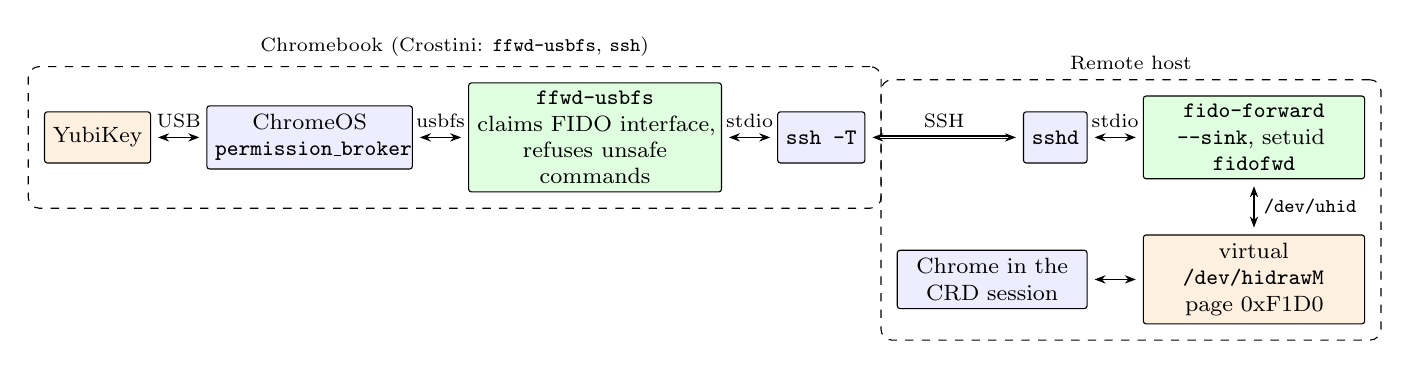
\begin{tikzpicture}[node distance=4mm and 7mm]
  \node[mem] (yk) {YubiKey};
  \node[sbox,right=of yk,text width=24mm] (pb) {ChromeOS\\\code{permission\_broker}};
  \node[act,right=of pb,text width=30mm] (src) {\code{ffwd-usbfs}\\claims FIDO interface,\\refuses unsafe commands};
  \node[sbox,right=of src] (ssh) {\code{ssh -T}};
  \node[sbox,right=20mm of ssh] (sshd) {\code{sshd}};
  \node[act,right=of sshd,text width=26mm] (sink) {\code{fido-forward}\\\code{--sink}, setuid\\\code{fidofwd}};
  \node[mem,below=7mm of sink,text width=26mm] (hid) {virtual \code{/dev/hidrawM}\\page 0xF1D0};
  \node[sbox,left=of hid,text width=22mm] (chr) {Chrome in the CRD session};
  \draw[bidi] (yk) -- node[above,font=\scriptsize]{USB} (pb);
  \draw[bidi] (pb) -- node[above,font=\scriptsize]{usbfs} (src);
  \draw[bidi] (src) -- node[above,font=\scriptsize]{stdio} (ssh);
  \draw[bidi,double] (ssh) -- node[above,font=\scriptsize]{SSH} (sshd);
  \draw[bidi] (sshd) -- node[above,font=\scriptsize]{stdio} (sink);
  \draw[bidi] (sink) -- node[right,font=\scriptsize]{\code{/dev/uhid}} (hid);
  \draw[bidi] (hid) -- (chr);
  \begin{scope}[on background layer]
    \node[draw,dashed,rounded corners,fit=(yk)(pb)(src)(ssh),inner sep=2mm,
          label={[font=\scriptsize]above:Chromebook (Crostini: \code{ffwd-usbfs}, \code{ssh})}] {};
    \node[draw,dashed,rounded corners,fit=(sshd)(sink)(hid)(chr),inner sep=2mm,
          label={[font=\scriptsize]above:Remote host}] {};
  \end{scope}
\end{tikzpicture}
\caption{Data flow of the recommended design. Only the FIDO interface leaves
the Chromebook. SSH is the only transport and the only authentication; no
TCP port opens on either host.}
\label{fig:flow}
\end{figure*}

\begin{example}[One login]
\label{ex:login}
\begin{enumerate}
\item Chrome on the remote host writes a \code{CTAPHID\_CBOR} request with
      \code{getAssertion} to \code{/dev/hidrawM}.
\item The sink reads it from \code{/dev/uhid} and sends the 64-byte reports
      up the SSH channel.
\item \code{ffwd-usbfs} joins the reports, checks the command against its
      policy, and writes them to the key's interrupt OUT endpoint.
\item The key sends keepalives until the user touches it, then the
      response.
\item \code{ffwd-usbfs} reads them from the interrupt IN endpoint and sends
      them down the SSH channel.
\item The sink writes them to \code{/dev/uhid}. Chrome reads the response
      and completes the login.
\end{enumerate}
\end{example}

Five reasons support this choice:
\begin{enumerate}
\item Only the FIDO interface leaves the Chromebook. PIV, OpenPGP and OTP
      stay local.
\item The relay refuses commands that erase or change the key
      (Section~\ref{sec:security}).
\item The remote half exists, drops privilege before it reads input, and
      builds with Bazel here for amd64 and arm64.
\item SSH is the only transport and authentication.
\item Keepalives pass through, so a slow touch does not time out.
\end{enumerate}

\subsection{OpenPGP and PIV: agent forwarding}

For OpenPGP, forward gpg-agent's extra socket with \code{RemoteForward}, and
run \code{scdaemon} and \code{pcscd} in Crostini~\cite{gnupgfwd}. For PIV,
run \code{p11-kit server} with the YubiKey PKCS\#11 module in Crostini and
forward its socket~\cite{p11kit}. The FIDO relay claims only the FIDO
interface, and \code{pcscd} claims only the CCID interface, so the two should
work side by side (assumption; test T6).

FIDO keys for SSH cannot be used from Crostini (Finding~\ref{find:nohidraw}).
On the remote host they work through the virtual key of approach B, because
the remote host has a \code{hidraw} node.

\subsection{Fallback: USB/IP with usbipdcpp}

Use approach A if the probe fails, or if you need PIV and OpenPGP as real
devices on the remote host. Use usbipdcpp, not jiegec/usbip. Use it only with
a remote host that you trust fully, because it gives that host's root user
full control of the key.

% SPDX-License-Identifier: Apache-2.0
\section{The new component}
\label{sec:component}

No existing tool reads a FIDO key through usbfs and relays it. The smallest
new component, \code{ffwd-usbfs}, fills that gap. Table~\ref{tab:component}
gives its design. We wrote it after the probe passed on a real Chromebook
(Section~\ref{sec:testplan}), and it passed the end-to-end test T4.

\begin{table}[t]
\centering
\caption{Design of \code{ffwd-usbfs}}
\label{tab:component}
\scriptsize
\begin{tabular}{@{}>{\raggedright\arraybackslash}p{15mm}>{\raggedright\arraybackslash}p{63mm}@{}}
\toprule
Item & Design \\
\midrule
Purpose & Key side of fido-forward for a host with a usbfs node and no \code{hidraw} node \\
Language & Go 1.27, \code{CGO\_ENABLED=0}, built with Bazel (\code{rules\_go}) \\
Libraries & \code{golang.org/x/sys/unix}, and the packages \code{ctaphid} and \code{usbfs} of this study \\
Command & \code{ffwd-usbfs [-d NODE] [--allow-management] HOST} \\
Transport & Starts \code{ssh -T HOST fido-forward --sink} with pipes, as fido-forward does; under \code{sudo} it gives up root before \code{ssh} starts \\
Wire & fido-forward v1: read \code{FFWD\textbackslash x01}, write it back, then raw 64-byte reports \\
USB & Find the HID interface with page 0xF1D0; detach \code{usbhid}; claim it; one reader of interrupt IN, one writer of interrupt OUT \\
Policy & Judge each request by its first packet; answer a refused CTAP2 command with status \code{0x27} (operation denied) and a refused vendor command with \code{CTAPHID\_ERROR}; drop the rest of the message; never send it to the key \\
Teardown & \code{CTAPHID\_CANCEL} on each channel, release, attach \code{usbhid} again \\
Size & 586 lines, and 214 lines of tests \\
\bottomrule
\end{tabular}
\end{table}

\subsection{Parts that exist now}

The study's workspace already holds the parts that need the most care. Both
are pure Go with unit tests, and both build with Bazel.

\paragraph{\code{ctaphid}} It splits a message into 64-byte reports and joins
them again. Its \code{Policy} type decides which CTAP2 commands pass.
Listing~\ref{lst:policy} shows the decision.

\begin{lstlisting}[style=go,caption={The command policy in package \code{ctaphid}},label={lst:policy},float=tb]
// Allowed: does the policy pass m to the key?
func (p Policy) Allowed(m Message) bool {
  if m.Command != CmdCBOR || len(m.Payload) == 0 {
    return true // framing (INIT, PING, CANCEL) or U2F
  }
  switch m.Payload[0] {
  case AuthMakeCredential, AuthGetAssertion, AuthGetInfo,
    AuthClientPIN, AuthGetNextAssertion, AuthSelection:
    return true
  case AuthReset, AuthCredentialManagement, AuthBioEnrollment,
    AuthConfig, AuthLargeBlobs, AuthCredMgmtPreview,
    AuthBioEnrollPreview:
    return p.AllowManagement
  default:
    return false // unknown commands are refused
  }
}
\end{lstlisting}

\paragraph{\code{usbfs}} It opens a usbfs node, parses the descriptors,
reads a HID report descriptor, detaches and attaches the kernel driver,
claims an interface, and runs interrupt transfers. A unit test checks that
each \code{ioctl} number that the code computes from its structure sizes
equals the number in \code{<linux/usbdevice\_fs.h>}.

\paragraph{\code{fido-probe}} It uses both packages. It finds the YubiKey,
detaches \code{usbhid} from the FIDO interface, sends \code{CTAPHID\_INIT}
and \code{getInfo}, and attaches the driver again. Both commands read only.

\paragraph{\code{relay}} It is the key side of fido-forward's wire
protocol. It has no USB code, so unit tests run it against a fake key. They
check that a reset of three packets never reaches the key, that the far side
gets status \code{0x27}, and that every used channel gets
\code{CTAPHID\_CANCEL} at the end.

\begin{tip}
The first version of \code{ffwd-usbfs} reads the interrupt IN endpoint in
a loop with a 200\,ms timeout. A later version can keep an IN transfer
pending at all times with asynchronous URBs (\code{USBDEVFS\_SUBMITURB} and
\code{USBDEVFS\_REAPURB}).
\end{tip}

% SPDX-License-Identifier: Apache-2.0
\section{Portability}
\label{sec:portability}

The relay has two sides, and each platform answers differently for each
side. The \term{key side} reads the real key. The \term{use side} makes a
virtual key for a browser. Table~\ref{tab:ports} gives the answers.

\begin{table}[t]
\centering
\caption{What each platform can do}
\label{tab:ports}
\scriptsize
\begin{tabular}{@{}>{\raggedright\arraybackslash}p{11mm}>{\raggedright\arraybackslash}p{33mm}>{\raggedright\arraybackslash}p{33mm}@{}}
\toprule
Platform & Key side & Use side \\
\midrule
Linux & Yes: \code{/dev/hidraw}, fido-forward's source as it is. & Yes: \code{/dev/uhid}, fido-forward's sink. \\
ChromeOS & Yes, if the probe passes: usbfs only (Finding~\ref{find:nohidraw}). & No: the Crostini kernel has no UHID or HIDRAW option~\cite{termina} (verified). \\
macOS & Yes: IOKit, pure Go through purego~\cite{usbhid}. & Hard: needs an entitlement that Apple must approve~\cite{iohidres} (verified). \\
\bottomrule
\end{tabular}
\end{table}

\subsection{macOS as the key side}

On macOS a process talks to a HID device through IOKit. The library
rafaelmartins/usbhid~\cite{usbhid} (BSD-3) calls IOKit through purego, so it
needs no cgo, and we cross-built it for both Mac CPUs with Bazel on Linux
(verified). It opens a device without seizing it. libfido2 seizes the device
instead~\cite{libfido2osx} (verified), so a relay built on libfido2 would
lock out the Mac's own browser. A relay that does not seize should let the
Mac's Chrome use the key at the same time (assumption; Chromium does not seize
either~\cite{libfido2osx}).

Two permission rules matter. macOS asks for Input Monitoring only for
keyboards, mice and touchpads, not for the FIDO interface~\cite{iohidfam}
(verified). A process that is not root can open the device only while its user
has a session at the Mac's screen~\cite{iohidfam} (verified). A relay that SSH
starts on a Mac therefore works while the user is logged in there.

\subsection{macOS and ChromeOS as the use side}

To make a virtual HID device, macOS requires the entitlement
\code{com.apple.developer.hid.virtual.device}, also for root~\cite{iohidres}
(verified). Apple grants it on request, after review, and one public request
waited 2.5 months. The program must then be a signed app with a provisioning
profile (assumption). DriverKit offers no shortcut: it needs Apple-granted
entitlements too. A Mac as the remote host can avoid this with approach E3, a
Chrome extension, which needs no entitlement but has the origin problem of
Section~\ref{sec:approaches}.

ChromeOS cannot be the use side. The Crostini kernel has no \code{uhid}
module, and Chrome on ChromeOS sees only the host's devices (assumption).

\subsection{What it takes}

\begin{itemize}
\item A key-side interface with four methods (open, read a report, write a
      report, close), and one implementation per platform, chosen by Go
      build tags. The probe already has this shape: \code{open\_linux.go}
      uses usbfs and \code{open\_darwin.go} uses IOKit.
\item The common client: the FFWD wire format, the command policy, and
      starting \code{ssh}. About 250 lines.
\item Bazel targets for each platform. One \code{bazel build //...} on Linux
      now builds the probe for Linux on amd64 and arm64 and for macOS on
      amd64 and arm64, all static and cgo free (verified).
\item For a Mac as the remote host: a signed Swift helper with the
      entitlement, Apple's approval, and a developer account.
\end{itemize}

The cheapest useful product has a key side on all three platforms and a use
side on Linux only. That covers a user who sits at a Chromebook or a Mac and
works on a Linux host.

% SPDX-License-Identifier: Apache-2.0
\section{Security}
\label{sec:security}

Table~\ref{tab:risks} lists the risks and their mitigations. The most
important one has no technical fix.

\begin{table}[t]
\centering
\caption{Risks and mitigations}
\label{tab:risks}
\scriptsize
\begin{tabular}{@{}>{\raggedright\arraybackslash}p{27mm}>{\raggedright\arraybackslash}p{6mm}>{\raggedright\arraybackslash}p{44mm}@{}}
\toprule
Risk & Where & Mitigation \\
\midrule
Remote erases the key or lists and deletes passkeys & B & The policy refuses commands 0x07, 0x09, 0x0A, 0x0C, 0x0D, 0x40, 0x41 and unknown ones. Reset also needs a touch soon after power-up~\cite{ctap21}. \\
Remote gets an assertion for a site you did not open & B, E3 & No technical fix. Run the relay only when you need it. Touch only for a login you started. Prefer passkeys with a PIN. \\
Remote guesses the FIDO PIN & B & The key limits PIN tries~\cite{ctap21}. \\
Remote root gets raw control of the key & A, E4 & Use B for FIDO. Use A only with a fully trusted host. \\
Other users on the remote host use the virtual key & B & fido-forward's udev rule gives the node to one group only. \\
The setuid sink is attacked & B & It drops privilege before it reads input and uses no cgo. Review its 610 lines before install. \\
A forwarded agent signs for any remote process & D & \code{ssh-add -c}, PIV touch policy, \code{ssh-add -h}~\cite{agentrestrict}; gpg restricts the extra socket. \\
\bottomrule
\end{tabular}
\end{table}

\begin{pitfall}[Phishing through the relay]
The relying party ID comes from Chrome on the remote host. The key shows no
site name. A compromised remote host can therefore ask the key for an
assertion for any site, and a touch approves it. The relay cannot tell a real
request from a forged one. Only the user's own judgement protects against
this, so the relay should run only while the user needs it.
\end{pitfall}

Approach B still keeps the damage smaller than approach A. Under B, a
compromised remote host can use the key's passkeys while the relay runs and
the user touches. Under A, it can also erase the PIV and OpenPGP applets and
change the OTP slots, without any touch.

% SPDX-License-Identifier: Apache-2.0
\section{Open questions and test plan}
\label{sec:testplan}

Tests T0 to T2 ran on a Chromebook on 2026-11-09, with a Google Titan key
in place of the YubiKey. The container saw the key only as a usbfs node with
mode \code{0664}, and no \code{hidraw} node. As root, the probe detached the
kernel driver, claimed the FIDO interface, and got a \code{CTAPHID\_INIT}
reply in 3\,ms. The Titan key speaks only U2F, so FIDO2 is still to be
tested with the YubiKey. Table~\ref{tab:tests} lists all the questions. The workspace file \code{TESTPLAN.md} gives the exact commands.

\begin{table}[t]
\centering
\caption{Open questions and tests}
\label{tab:tests}
\scriptsize
\begin{tabular}{@{}l>{\raggedright\arraybackslash}p{50mm}l@{}}
\toprule
\# & Question & Test \\
\midrule
Q1 & Does ChromeOS share the YubiKey with Linux on this model? & T1 \\
Q2 & Does the container see the usbfs node, and with which mode? & T1: yes, 0664 \\
Q3 & Can the container detach \code{usbhid}, claim the FIDO interface, and run CTAPHID? & T2: yes, as root \\
Q4 & Is the Chromebook amd64 or arm64? & T0: amd64 \\
Q5 & Does SSH latency stay far below Chrome's 20\,s device timeout? & T5 \\
Q6 & Can \code{pcscd} hold the CCID interface while the relay runs? & T6 \\
Q7 & Can Chrome in the CRD session open the virtual \code{hidraw} node? & T4 \\
Q8 & Does the key return to ChromeOS when sharing stops? & T7 \\
Q9 & Must the Smart Card Connector app be off? & T1 \\
\bottomrule
\end{tabular}
\end{table}

The order matters. T1 and T2 decide whether approaches A and B can work at
all, and they take about ten minutes. The probe needs no installation in
\code{penguin}, because Bazel builds it as a static binary.

\begin{lstlisting}[style=shell,caption={Tests T0 to T2},label={lst:probe},float=tb]
# build host, in the workspace; pick the Chromebook's CPU
bazel build \
  //cmd/fido-probe:fido-probe_linux_amd64
# penguin, after sharing the key in Manage USB devices
uname -m
ls -l /dev/bus/usb/*/* /dev/hidraw*
sudo ./fido-probe_linux_amd64
# expected last line:
# PASS: the FIDO interface works from this machine
\end{lstlisting}

If T1 fails, ChromeOS refuses the key, and only approach E5 remains. If T2
fails with \code{operation not permitted}, the container cannot detach the
driver, and approaches A and B both fail on that Chromebook.

% SPDX-License-Identifier: Apache-2.0
\section{Conclusion}
\label{sec:conclusion}

Chrome Remote Desktop does not forward security keys, and it cannot be
changed. The way to use a Chromebook's YubiKey on a remote Linux desktop is
to relay the key's FIDO channel over SSH into a virtual FIDO key that
\code{uhid} creates on the remote host.

One fact shapes the design. The ChromeOS Linux container receives a shared
key only as a usbfs node, so every existing relay, which reads
\code{hidraw}, fails there. A small new key-side program that reads the key
through usbfs closes the gap. It reuses fido-forward's remote half and adds a
policy that refuses commands that can erase or change the key. OpenPGP and
PIV use agent forwarding instead.

The probe on a real Chromebook answered the one question that source code
could not: the container can claim a security key's FIDO interface, as root.
A YubiKey~5 answered FIDO~2.1 requests through it. The remaining work is
about 400 lines of Go for the relay.


% IEEEtran: \appendices starts the appendix sections (A, B, ...).
\appendices
% SPDX-License-Identifier: Apache-2.0
\section{How a YubiKey works}
\label{app:yubikey}

This appendix explains the parts of a YubiKey that the study depends on.
It covers the YubiKey 5 series. Older models differ in details.

\subsection{One device, several applications}

A YubiKey holds several independent applications. Each one has its own keys,
its own PIN or password, and its own reset. Resetting the FIDO application
does not touch the PIV keys, and the reverse. Each application is reached
through one of the three USB interfaces in Table~\ref{tab:interfaces}.
Table~\ref{tab:apps} lists the applications.

\begin{table}[t]
\centering
\caption{YubiKey 5 applications}
\label{tab:apps}
\scriptsize
\begin{tabular}{@{}>{\raggedright\arraybackslash}p{13mm}>{\raggedright\arraybackslash}p{9mm}>{\raggedright\arraybackslash}p{24mm}>{\raggedright\arraybackslash}p{24mm}@{}}
\toprule
Application & USB interface & What it stores & How it proves \\
\midrule
FIDO U2F and FIDO2 & FIDO HID & a master key; discoverable credentials & signs a challenge after a touch \\
Yubico OTP & OTP HID (keyboard) & an AES-128 key and counters & types a 44-character one-time password \\
PIV & CCID & up to 24 key slots with certificates & signs or decrypts after a PIN \\
OpenPGP & CCID & signature, encryption and authentication keys & signs, decrypts or authenticates after a PIN \\
OATH & CCID & TOTP and HOTP secrets & computes a code for an app on the host \\
\bottomrule
\end{tabular}
\end{table}

The keys are made inside the YubiKey, and the device has no command that
exports a private key. A host can only ask the key to use a private key, for
example to sign. This is the reason why approach~C cannot work: a virtual
authenticator on the remote host cannot borrow the real key's private keys.

\subsection{FIDO credentials}

A FIDO credential is a key pair for one site, the \term{relying party}.
WebAuthn defines two operations~\cite{webauthn3}. Figure~\ref{fig:webauthn}
shows them.

\begin{figure}[t]
\centering
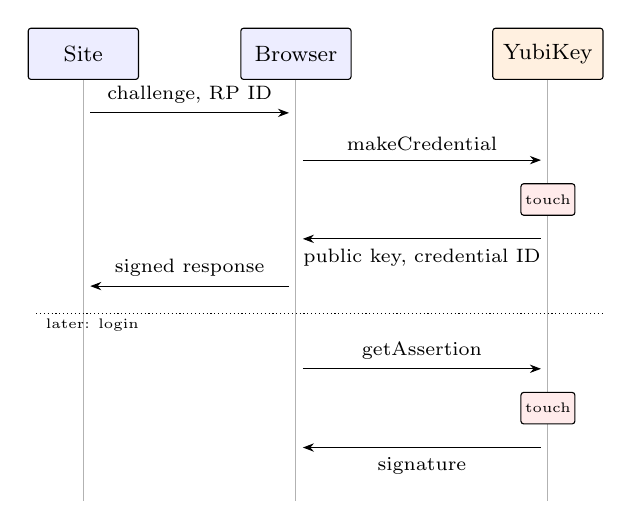
\begin{tikzpicture}[font=\scriptsize]
  \node[sbox,minimum width=14mm] (rp) at (0,0) {Site};
  \node[sbox,minimum width=14mm] (br) at (2.7,0) {Browser};
  \node[mem,minimum width=14mm] (yk) at (5.9,0) {YubiKey};
  \foreach \n in {rp,br,yk} \draw[black!30] (\n.south) -- ++(0,-5.35);
  \draw[fl] (0,-0.75) -- node[above]{challenge, RP ID} (2.7,-0.75);
  \draw[fl] (2.7,-1.35) -- node[above]{makeCredential} (5.9,-1.35);
  \node[warnb,font=\tiny,minimum height=4mm,inner sep=1.5pt] at (5.9,-1.85) {touch};
  \draw[fl] (5.9,-2.35) -- node[below]{public key, credential ID} (2.7,-2.35);
  \draw[fl] (2.7,-2.95) -- node[above]{signed response} (0,-2.95);
  \draw[densely dotted] (-0.6,-3.3) -- (6.6,-3.3);
  \node[anchor=west,font=\tiny] at (-0.6,-3.45) {later: login};
  \draw[fl] (2.7,-4.0) -- node[above]{getAssertion} (5.9,-4.0);
  \node[warnb,font=\tiny,minimum height=4mm,inner sep=1.5pt] at (5.9,-4.5) {touch};
  \draw[fl] (5.9,-5.0) -- node[below]{signature} (2.7,-5.0);
\end{tikzpicture}
\caption{Registration (top) and login (bottom). The browser sends the
challenge and the RP ID to the key; the key signs only after a touch.}
\label{fig:webauthn}
\end{figure}

\paragraph{Registration} The browser sends \code{makeCredential} with the
site's RP ID, a hash of the client data (which holds the site's challenge
and origin), and the user. After a touch, the key makes a new key pair. It
returns the public key and a \term{credential ID}, signed with its
attestation key.

\paragraph{Login} The browser sends \code{getAssertion} with the RP ID, a
new client data hash, and the credential IDs that the site knows. After a
touch, the key signs the authenticator data and the client data hash with
the credential's private key. The authenticator data holds a hash of the RP
ID, flags for user presence and user verification, and a signature counter.

\paragraph{Where the private key lives} A YubiKey makes a new key pair for
each registration. For a \term{non-discoverable} credential, it encrypts the
private key and some metadata with a master key that is unique to that
YubiKey and never leaves it. The result is the credential ID, which the site
stores~\cite{yk-keygen} (verified, firmware 4.4 and later). At login, the
site sends the credential ID back, and only the same YubiKey can decrypt it.
Such credentials therefore use no storage on the key. A
\term{discoverable} credential, also called a resident key or a passkey, is
stored on the key with the site's user handle, so a login needs no user
name~\cite{yk-resident} (verified). The key has room for a limited number of
these.

\paragraph{Presence and verification} A touch proves \term{user presence}: a
person is at the key. A PIN proves \term{user verification}: the right person
is at the key. The PIN is checked by the key itself, not by the host. Both
flags are part of the signed data, so the site can check them.

\paragraph{Why a phishing site gets no usable signature} The signed
data contains a hash of the RP ID, and the client data contains the origin.
A phishing site with a different name gets a signature that the real site
rejects. The browser chooses the RP ID. That is the reason why a relay that
trusts a compromised remote browser cannot stop phishing
(Section~\ref{sec:security}).

\subsection{Yubico OTP}

The OTP application acts as a USB keyboard. A touch makes it type a
44-character password~\cite{yk-otp} (verified). The first 12 characters are
the key's public ID, and they never change. The other 32 characters are
fields encrypted with the key's AES-128 key. The fields include a usage
counter and a session counter, so a server rejects a password that was used
before. The characters come from a small alphabet, called modhex, that types
the same on most keyboard layouts. The OTP application is not a goal of
this study.

\subsection{PIV}

PIV is a smart card standard from the US government. A YubiKey 4 or 5 has 24
PIV slots, and each holds a private key and an X.509
certificate~\cite{yk-piv} (verified). Four slots have defined uses:
\begin{itemize}
\item 9a, authentication: for example system login. One PIN entry permits
      many operations.
\item 9c, digital signature: the PIN is needed before every signature.
\item 9d, key management: decryption, for example of e-mail.
\item 9e, card authentication: for example physical access.
\end{itemize}
The PIN policy can be changed, and a slot can also ask for a touch. Hosts
reach PIV through the CCID interface, with PC/SC and a PKCS\#11 module. This
is the path that p11-kit forwards in approach~D.

\subsection{OpenPGP}

The OpenPGP application is an OpenPGP smart card~\cite{yk-pgp}. It holds up
to three keys: one to sign, one to decrypt, and one to authenticate. GnuPG
uses it through \code{scdaemon} and the CCID interface. A forwarded
gpg-agent lets a remote host ask for a signature, while the PIN entry and the
touch stay on the Chromebook (approach~D).

\subsection{What this means for forwarding}

Each application sits on one USB interface. A relay that forwards one
interface forwards only the applications behind it. The recommended relay
forwards the FIDO interface, so a compromised remote host can use FIDO
credentials while the relay runs, and nothing else. USB/IP forwards all
three interfaces, so the remote host can also use, or reset, the PIV and
OpenPGP applications and change the OTP configuration.


% =====================================================================
\begin{thebibliography}{30}
\bibitem{ctap21} FIDO Alliance, ``Client to Authenticator Protocol (CTAP), version 2.1,''
  Proposed Standard, Jun. 2021. \url{https://fidoalliance.org/specs/fido-v2.1-ps-20210615/fido-client-to-authenticator-protocol-v2.1-ps-20210615.html}
\bibitem{ctap22} FIDO Alliance, ``Client to Authenticator Protocol (CTAP), version 2.2,''
  Jul. 2025, section ``Hybrid''. \url{https://fidoalliance.org/specs/fido-v2.2-ps-20250714/fido-client-to-authenticator-protocol-v2.2-ps-20250714.html}
\bibitem{webauthn3} W3C, ``Web Authentication, Level 3,'' section ``Relying Party Identifier''.
  \url{https://www.w3.org/TR/webauthn-3/}
\bibitem{yk-usb} Yubico, ``YubiKey 5 USB interfaces,'' YubiKey Technical Manual.
  \url{https://docs.yubico.com/hardware/yubikey/yk-tech-manual/yk5-usb-interface.html}
\bibitem{tremplin} ChromiumOS, \code{tremplin}, \code{src/chromiumos/tremplin/start\_lxd.go},
  lines 192 to 228 and 366, commit 744f7e4.
\bibitem{pb} ChromiumOS, \code{permission\_broker},
  \code{allow\_conforming\_usb\_device\_rule.cc}.
  \url{https://chromium.googlesource.com/chromiumos/platform2/+/HEAD/permission_broker/}
\bibitem{crosusb} Chromium, \code{chrome/browser/ash/usb/cros\_usb\_detector.cc}.
  \url{https://chromium.googlesource.com/chromium/src/+/main/chrome/browser/ash/usb/cros_usb_detector.cc}
\bibitem{crosvmdev} crosvm-dev mailing list, thread D5iCnoTk-4k on \code{vmc usb-attach} and \code{vmc key-attach}, Jul. to Aug. 2025.
  \url{https://groups.google.com/a/chromium.org/g/crosvm-dev/c/D5iCnoTk-4k}
\bibitem{cros-scc} chromium-os-dev mailing list, threads on Smart Card Connector and
  USB sharing, 2020 and 2025.
  \url{https://groups.google.com/a/chromium.org/g/chromium-os-dev/c/2bVDprdrLOY}
\bibitem{devio} Linux kernel, \code{drivers/usb/core/devio.c}.
  \url{https://github.com/torvalds/linux/blob/master/drivers/usb/core/devio.c}
\bibitem{chromefido} Chromium, \code{device/fido/hid/fido\_hid\_discovery.cc},
  \code{fido\_hid\_device.cc}, and \code{device/fido/public/fido\_constants.cc}.
\bibitem{crdpol} Chromium, policy definitions \code{RemoteAccessHostAllowGnubbyAuth},
  \code{WebAuthenticationRemoteProxiedRequestsAllowed},
  \code{WebAuthenticationRemoteDesktopAllowedOrigins}.
\bibitem{wap} Chrome for Developers, ``\code{chrome.webAuthenticationProxy}.''
  \url{https://developer.chrome.com/docs/extensions/reference/api/webAuthenticationProxy}
\bibitem{fidoforward} txomon (GitHub), \code{fido-forward}, commit 2b7b2ac, Oct. 2026, MIT license.
  \url{https://github.com/txomon/fido-forward}
\bibitem{qubes} QubesOS, \code{qubes-app-u2f}, commit 069a20b, Oct. 2026, GPL-2.0+.
  \url{https://github.com/QubesOS/qubes-app-u2f}
\bibitem{jiegec} jiegec (GitHub), \code{usbip}, Rust crate, commit d5774284, MIT license.
  \url{https://github.com/jiegec/usbip}
\bibitem{usbipdcpp} yunsmall (GitHub), \code{usbipdcpp}, commit 00f4509, LGPL-3.0.
  \url{https://github.com/yunsmall/usbipdcpp}
\bibitem{virtualfido} Bulwark ID, \code{virtual-fido}, commit 512d8a3, Jun. 2024, MIT license.
  \url{https://github.com/bulwarkid/virtual-fido}
\bibitem{authrelay} Parallel Works, \code{auth-relay}, commit 851f1e9, May 2026.
  \url{https://github.com/parallelworks/auth-relay}
\bibitem{vsmartcard} F.~Morgner, \code{vsmartcard}, commit 93286a9, Oct. 2026, GPL-3.0.
  \url{https://github.com/frankmorgner/vsmartcard}
\bibitem{openssh} OpenBSD, OpenSSH release notes 8.2, 8.4, 8.9 and 9.3p2, and the
  \code{ssh-agent(1)} and \code{ssh-add(1)} manual pages. \url{https://www.openssh.com/releasenotes.html}
\bibitem{agentrestrict} OpenSSH, ``SSH agent restriction.'' \url{https://www.openssh.org/agent-restrict.html}
\bibitem{gnupgfwd} GnuPG wiki, ``AgentForwarding.'' \url{https://wiki.gnupg.org/AgentForwarding}
\bibitem{p11kit} p11-kit, ``Sharing PKCS\#11 modules with p11-kit,'' manual, release 0.26.5, BSD-3-Clause.
  \url{https://p11-glue.github.io/p11-glue/p11-kit/manual/remoting.html}
\bibitem{systemd} systemd, \code{src/udev/fido\_id/fido\_id.c} and \code{rules.d/60-fido-id.rules}.
  \url{https://github.com/systemd/systemd}
\bibitem{yk-keygen} Yubico, ``U2F key generation,'' developer documentation.
  \url{https://developers.yubico.com/U2F/Protocol_details/Key_generation.html}
\bibitem{yk-resident} Yubico, ``Discoverable credentials / resident keys,'' WebAuthn developer guide.
  \url{https://developers.yubico.com/WebAuthn/WebAuthn_Developer_Guide/Resident_Keys.html}
\bibitem{yk-otp} Yubico, ``OTPs explained,'' developer documentation.
  \url{https://developers.yubico.com/OTP/OTPs_Explained.html}
\bibitem{yk-piv} Yubico, ``PIV certificate slots,'' developer documentation.
  \url{https://developers.yubico.com/PIV/Introduction/Certificate_slots.html}
\bibitem{yk-pgp} Yubico, ``OpenPGP,'' developer documentation. \url{https://developers.yubico.com/PGP/}
\bibitem{usbhid} rafaelmartins (GitHub), \code{usbhid}, module \code{rafaelmartins.com/p/usbhid}, Oct. 2026, BSD-3-Clause.
  \url{https://github.com/rafaelmartins/usbhid}
\bibitem{libfido2osx} Yubico, libfido2 \code{src/hid\_osx.c} (lines 201, 451), and Chromium
  \code{services/device/hid/hid\_service\_mac.cc} (line 175).
\bibitem{iohidfam} Apple, IOHIDFamily, \code{IOHIDDevice.cpp} (lines 527 to 531) and
  \code{IOHIDLibUserClient.cpp} (lines 332, 710 to 714).
  \url{https://github.com/apple-oss-distributions/IOHIDFamily}
\bibitem{iohidres} Apple, IOHIDFamily, \code{IOHIDResourceUserClient.cpp} (lines 32 to 33 and 117 to 148),
  and ``com.apple.developer.hid.virtual.device,'' developer documentation.
\bibitem{termina} ChromiumOS kernel, \code{chromeos/config/termina/base.config}, chromeos-6.6, commit c3031f3e.
\bibitem{usbip-deb} Debian, package \code{usbip}, trixie. \url{https://packages.debian.org/trixie/usbip}
\end{thebibliography}

\end{document}
